% vim: set spell spelllang=es syntax=tex :

\section{Clasificación de los modelos de cómputo paralelos}

\label{mt_modelosparalelos}

Existen varias formas de clasificar los modelos computacionales, en esta
sección nos enfocaremos en aquellas dos que son de particular interés para éste
trabajo: la clasificación de Flynn, que compara la relación entre los flujos de
datos y los de instrucciones, y la clasificación según los modelos de memoria
compartida y distribuida, que analiza la forma en la que las unidades de
procesamiento comparten datos.

\subsection{Taxonomía de Flynn}

La taxonomía de Flynn \cite{flynnstaxonomy1972} propone describir la estructura
general de una arquitectura según la magnitud de interacción de los flujos de
datos e instrucciones. Esto permite definir cuatro clases distintas:

\begin{description}

	\item[Single Instruction stream/Single Data stream (\emph{SISD}):] En
		este modelo solo hay un flujo de instrucciones que opera sobre
		un único flujo de datos. Éste modelo se corresponde con la
		arquitectura de Von Neumann.

	\item[Single Instruction stream/Multiple Data stream (\emph{SIMD}):] En
		este modelo solo hay un flujo de instrucciones que opera sobre
		varios flujos de datos al mismo tiempo. Para poder ejecutar los
		distintos flujos de instrucciones, las computadoras que
		implementan este modelo tienen varias unidades de procesamiento
		que comparten la misma unidad de control. En un ciclo de
		instrucción, todas las unidades de procesamiento ejecutan la
		misma instrucción sobre distintos elementos de datos. Algunas
		implementaciones de este modelo agregan un bit de actividad
		asociado a cada unidad de procesamiento que indica si debe
		ejecutar la instrucción o no operar. Esta extensión permite
		implementar estructuras condicionales con facilidad pero
		reduciendo la performance \cite{introToPC2002}. Éste modelo es
		el utilizado en las placas aceleradoras modernas.

	\item[Multiple Instruction stream/Single Data stream (\emph{MISD}):] En
		este modelo múltiples flujos de instrucciones operan sobre un
		único flujo de datos. Si todas las unidades de procesamiento
		ejecutan el mismo conjunto de instrucciones, este modelo puede
		ser utilizado con el fin de aumentar la redundancia. Los
		sistemas de vuelo críticos del transbordador espacial STS
		implementaron este modelo con éste propósito
		\cite{spaceShuttlePCS1984}. En una alteración del modelo solo la
		primera unidad de procesamiento lee del conjunto de datos,
		mientras que el resto de las unidades tienen como datos de
		entrada los producidos por la inmediatamente anterior. Las
		\emph{tuberías} de los sistemas \emph{UNIX} pueden verse como
		una implementación de la extinción del modelo \emph{MISD}.

	\item[Multiple Instruction stream/Multiple Data stream (\emph{MIMD}):] En
		este modelo múltiples flujos de instrucciones operan sobre
		múltiples flujos de datos. Al igual que las computadoras
		\emph{SIMD}, las \emph{MIMD}, tienen múltiples unidades de
		procesamiento, cada una con su propia unidad de control.
		Lo que incrementa el costo y consumo energético
		\cite{introToPC2002}. Los sistemas multiprocesador de las
		computadoras de escritorio convencionales implementan este
		modelo.

\end{description}

\subsection{Memoria compartida y memoria distribuida}

Una característica importante de los sistemas \emph{MIMD} es la manera en la
cual las unidades de procesamiento pueden acceder a los datos de las demás,
dependiendo de si todas las unidades de procesamiento comparten el mismo espacio
de direcciones o si existe un espacio de direcciones asociado a cada conjunto de
unidades de procesamiento \cite{introToPC2002, anIntroToPP2011}:

\begin{description}

	\item[Memoria compartida:] Solo hay un espacio de memoria para todas las
		unidades. Para la comunicación los hilos de ejecución pueden
		utilizar memoria compartida, permitiendo comunicación
		implícita. También admiten comunicación por paso de mensajes. El
		espacio de memoria puede estar dividido en distintos bancos de
		memoria asociados a distintos conjuntos de unidades de
		procesamiento. Si el tiempo de acceso a los bancos de memoria es
		independiente de la unidad de procesamiento que realiza el
		acceso, la arquitectura es clasificada como de \emph{acceso a
		memoria uniforme}, abreviado como \emph{UMA} (del Inglés
		\emph{Uniform Memory Access}). Si el tiempo de acceso depende de
		la unidad de procesamiento y el banco al que se quiere acceder,
		la arquitectura es clasificada como de \emph{acceso a memoria no
		uniforme}, abreviado como \emph{NUMA} (del Inglés \emph{Non
		Uniform Memory Access}). Las computadoras multiprocesador de
		escritorio actuales son sistemas de memoria compartida
		\emph{UMA}. En la figura \ref{memCompartida} se muestra la
		arquitectura de memoria compartida.

\begin{figure}[!htb]

	\centering
	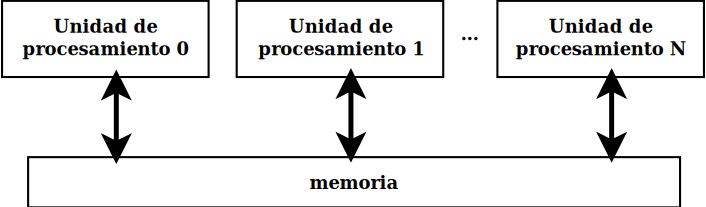
\includegraphics[width=0.9\textwidth]{img/memCompartida.pdf}
	\caption{Arquitectura de una maquina de memoria compartida.}

	\label{memCompartida}

\end{figure}

	\item[Memoria distribuida:] Cada unidad de procesamiento tiene su propio
		banco de memoria y su propio espacio de direcciones. La
		comunicación entre los hilos ejecutando en distintas unidades de
		procesamiento se realiza a través de paso de mensajes, por lo
		que toda la comunicación es explicita y controlada por el
		programador. El acceso a la memoria local es mucho más rápido
		que el acceso a los datos de otra unidad de procesamiento, y
		dependiendo de la red de comunicación puede variar entre
		distintos nodos. En la figura \ref{memDistribuida} se puede ver
		las conexión entre memorias y unidades de procesamiento en un
		sistema de memoria distribuida.

\begin{figure}[!htb]

	\centering
	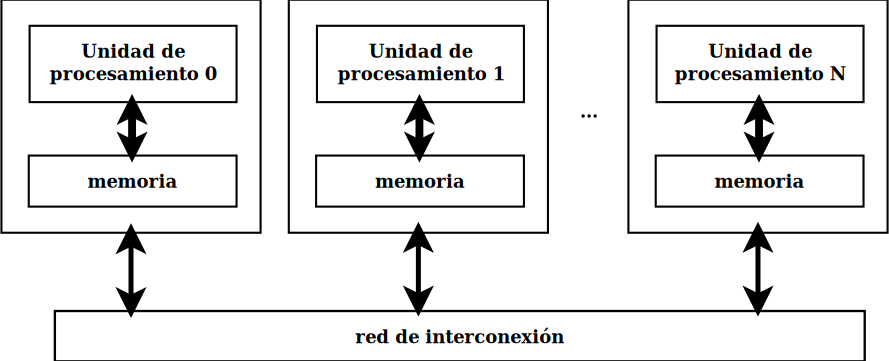
\includegraphics[width=0.9\textwidth]{img/memDistribuida.pdf}
	\caption{Arquitectura de una maquina de memoria distribuida.}

	\label{memDistribuida}

\end{figure}


	\item[Sistemas híbridos:] Son sistemas de memoria distribuida donde
		cada unidad de procesamiento es en realidad un sistema de
		memoria compartida. En la figura \ref{memHibrida} se muestra las
		distintas conexiones entre los bancos de memorias y las unidades
		de procesamiento.

\begin{figure}[!htb]

	\centering
	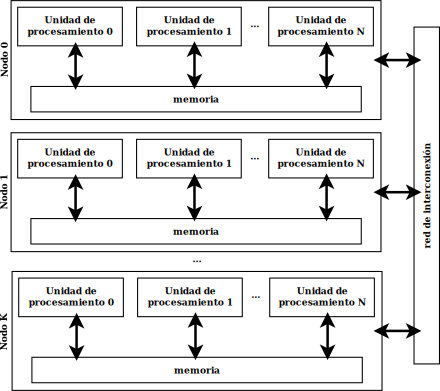
\includegraphics[width=0.9\textwidth]{img/memHibrida.pdf}
	\caption{Arquitectura de una maquina de memoria híbrida.}

	\label{memHibrida}

\end{figure}

\end{description}
